\documentclass{article}

\usepackage[T2A]{fontenc}
\usepackage[main=russian,english]{babel}
\usepackage{amsmath}
\usepackage{booktabs}
\usepackage{makecell}
\usepackage{multirow}
\usepackage{multicol}
\usepackage[normalem]{ulem}
\usepackage{xurl}  
\usepackage{dan2e}
\usepackage[hidelinks]{hyperref}

% Эти четыре строчки, чтобы исправить проблему с компиляцией 
% т.к. не определялся if@Russian, возможно из-за более новой версии babel
\makeatletter
\@ifundefined{@Russian}{\newif\if@Russian \@Russiantrue}{}
\@ifundefined{@TVP}     {\newif\if@TVP    \@TVPfalse}{}
\makeatother

\begin{document}
\raggedbottom
\Volume{ }
\Year{2025}
\Pages{ }

\udk{004.8}

\title{RuWikiBench: оценка больших языковых моделей посредством воспроизведения энциклопедических статей}

\author{Д.\,А.~Григорьев\Addressmark[1]\Emailmark[1], Д.\,И.~Чернышев\Addressmark[1]\Emailmark[2]}

\Addresstext[1]{Московский государственный университет им.~М.\,В.~Ломоносова, Москва, Россия}

\Emailtext[1]{dagrig14@yandex.ru}

\Emailtext[2]{chdanorbis@yandex.ru}

\markboth{Д.\,А.~Григорьев, Д.\,И.~Чернышев}{RuWikiBench: оценка больших языковых моделей}

\presentedby{...}

\dateA{ }
\dateB{ }
\dateC{ }

\alttitle{RuWikiBench: Evaluating Large Language Models through replication of encyclopedia articles}

\altauthor{D.\,A.~Grigoriev\Addressmark[a]\Emailmark[1], D.\,I.~Chernyshev\Addressmark[a]\Emailmark[2]}

\altAddresstext[a]{Lomonosov Moscow State University, Moscow Center for Fundamental and Applied Mathematics, Moscow, Russian Federation}

\altpresentedby{...}

\maketitle

\begin{abstract}
В связи с растущим интересом к использованию больших языковых моделей (LLM) в качестве инструментов для генерации научных текстов, 
оценка их способностей к созданию энциклопедического контента становится все более актуальной.
Однако для русскоязычных материалов этот вопрос изучен недостаточно, а существующие бенчмарки не охватывают ключевых аспектов аналитической работы с источниками.
В данной работе представлен RuWikiBench - открытый бенчмарк на основе <<Рувики>> для оценки способностей больших языковых моделей воспроизводить статьи в стиле Википедии, 
основанный на трех задачах: отбор релевантных источников, построение структуры статьи и генерация секций.
Результаты тестирования популярных открытых LLM показывают, что даже в идеальных условиях лучшие модели не всегда следуют экспертной логике составления энциклопедических материалов. 
\end{abstract}

\begin{keywords}
бенчмарк, Википедия, Рувики, большие языковые модели
\end{keywords}

\begin{altabstract}
In light of the growing interest in using large language models (LLMs) as tools for generating scientific texts,
the evaluation of their ability to produce encyclopedic content is becoming increasingly relevant.
However, for Russian-language materials this issue has not been sufficiently studied, and existing benchmarks do not cover key aspects of analytical work with sources.
This paper presents RuWikiBench - an open benchmark based on <<Ruwiki>> for evaluating the ability of large language models to reproduce Wikipedia-style articles,
built around three tasks:
selection of relevant sources, article structuring, and section generation.
The results of testing popular open-source LLMs show that even under ideal conditions, the best models do not always follow the expert logic of composing encyclopedic content.
\end{altabstract}

\begin{altkeywords}
benchmark, Wikipedia, Ruwiki, large language model
\end{altkeywords}

% ВВЕДЕНИЕ --------
\section*{Введение}

Современные большие языковые модели демонстрируют впечатляющие результаты в генерации текстов различной стилистики и тематики. 
Однако их способности к работе с научными и энциклопедическими материалами остаются малоизученными, особенно для русскоязычных текстов.
Существующие методы оценки способностей моделей преимущественно фокусируются на стандартных лингвистических задачах, не уделяя достаточного внимания аналитическим способностям при работе с научными текстами.
Для русского языка эта проблема особенно актуальна из-за ограниченной доступности специализированных оценочных инструментов.

Существует множество бенчмарков, охватывающих различные лингвистические задачи для русского языка.
RussianSuperGlue \cite{rsglue} оценивает общее языковое понимание и базовые задачи по обработке естественного языка. 
MERA \cite{mera} обеспечивает единые условия тестирования моделей за счет составления инструкций к генерации для каждой задачи, однако сами задачи ориентированы на проверку общего понимания. 
LIBRA \cite{libra} фокусируется на проверке способности модели к удержанию и извлечению информации из большого контекста, но сосредоточен на коротких ответах, не требующих глубоких рассуждений. 
Ru Arena General \cite{arena} фокусируется на парном сравнении моделей, но не на общем качестве ответа.
Ping-Pong \cite{pp} оценивает диалоговые способности моделей, что важно для интерактивных систем, но не подходит для оценки способности проводить исследования и писать связные научно-энциклопедические тексты.
При этом остается неохваченным целый класс задач, связанных с глубоким анализом текстов: создание развернутых, структурированных и фактологически точных текстов, подкрепленных большим количеством источников. 

Недавнее развитие новых способностей агентов, например появление функции <<Deep Research>> у OpenAI \cite{deepr} или разработка универсального алгоритма Storm \cite{storm}, 
свидетельствует о возрастающем интересе к проведению научных исследований с помощью больших языковых моделей, 
что говорит о необходимости создания новых подходов к объективной оценке аналитических способностей моделей. 
Существующие бенчмарки в ограниченной степени затрагивают критически важные для генерации научно-энциклопедических текстов аспекты, 
такие как умение обобщать информацию из набора документов, планировать структуру будущего текста, соблюдать связанность и логическую последовательность изложения, а также обеспечивать точность и достоверность фактов. 
Одним из наиболее близких исследований в этой области является бенчмарк ResearchArena \cite{resar}, в котором формализуют построение академического обзора, 
однако он больше нацелен на проверку способности моделей отбирать и организовывать релевантную информацию и не затрагивает способность моделей генерировать связные научно-энциклопедические тексты.

В данной работе предлагается подход, направленный на создание 
инструментов, позволяющих тестировать, насколько большие языковые модели умеют работать с научно-энциклопедическими текстами.
В рамках исследования:
\begin{enumerate}

    \item Собран размеченный набор данных на основе интернет-энциклопедии <<Рувики>>;
    
    \item Разработан открытый бенчмарк RuWikiBench, позволяющий измерять качество модели на задачах, требующих глубокого анализа текста;
    
    \item Протестированы способности лучших открытых больших языковых моделей порождать статьи в стиле Википедии.

\end{enumerate}

Код и данные работы выложены в открытый доступ\footnote{\url{https://github.com/Nejimaki-Tori/WikiBench}}.

% СБОР ДАННЫХ --------
\section*{Сбор данных}

Для построения бенчмарка, направленного на оценку способности языковых моделей к работе с источниками к статьям, необходимо подготовить корпус текстов, который будет использоваться в генерации. 
Выбор сделан в пользу стилистики Википедии по той причине, что этот жанр одновременно требует фактологической точности, полноты анализа и понимания контекста, что хорошо соотносится с направлением исследования этой работы.

В качестве источника была выбрана российская интернет-энциклопедия <<Рувики>>, которая отличается большим числом ссылок на русскоязычные источники, а также более строгой фильтрацией текстов, 
что позволяет положиться на нее как на надежный эталон для оценки качества генерации русскоязычных статей.

Процесс получения данных включал следующие шаги:

\begin{enumerate}

    \item \textbf{Выбор статей}: вручную были отобраны статьи на разнообразные темы, содержащие достаточное количество ссылок на внешние источники;
    
    \item \textbf{Загрузка источников}: для каждой статьи были автоматически собраны доступные источники, на которые она ссылается;
    
    \item \parbox[t]{0.9\textwidth}{\textbf{Разбиение на сниппеты}: для воспроизведения реальных условий Retrieval Augmented Generation (RAG), все тексты были разбиты на небольшие фрагменты длиной $\approx 600$ слов.}

\end{enumerate}

\begin{figure}[ht!]
  \centering
  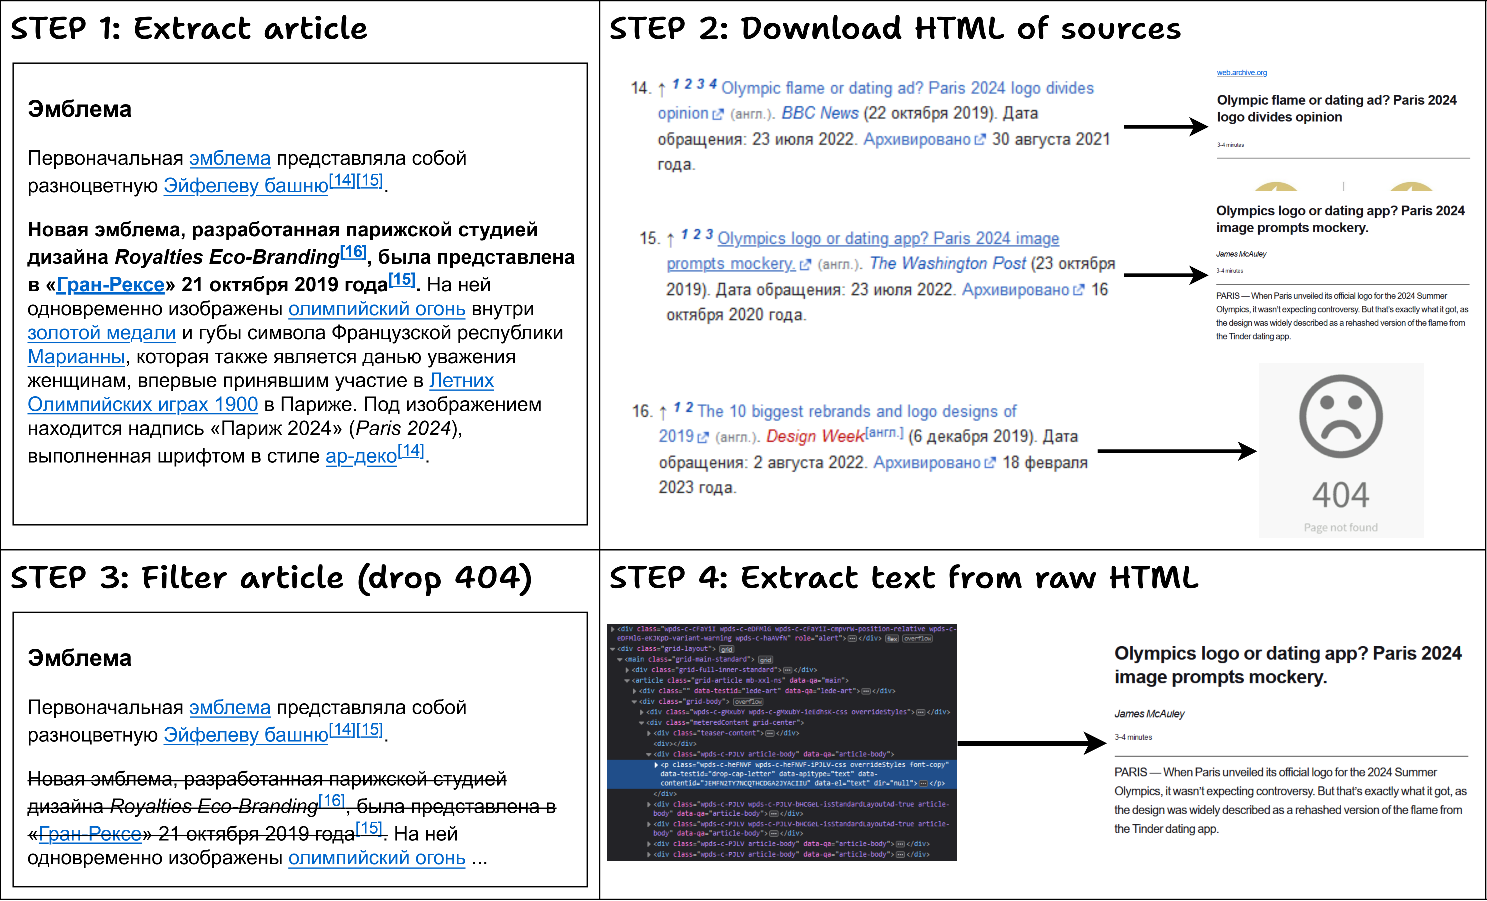
\includegraphics[width=0.9\textwidth]{figures/Source_extract.png}
  \caption{Извлечение источников}
  \label{fig:source}
\end{figure}

\begin{figure}[ht!]
  \centering
  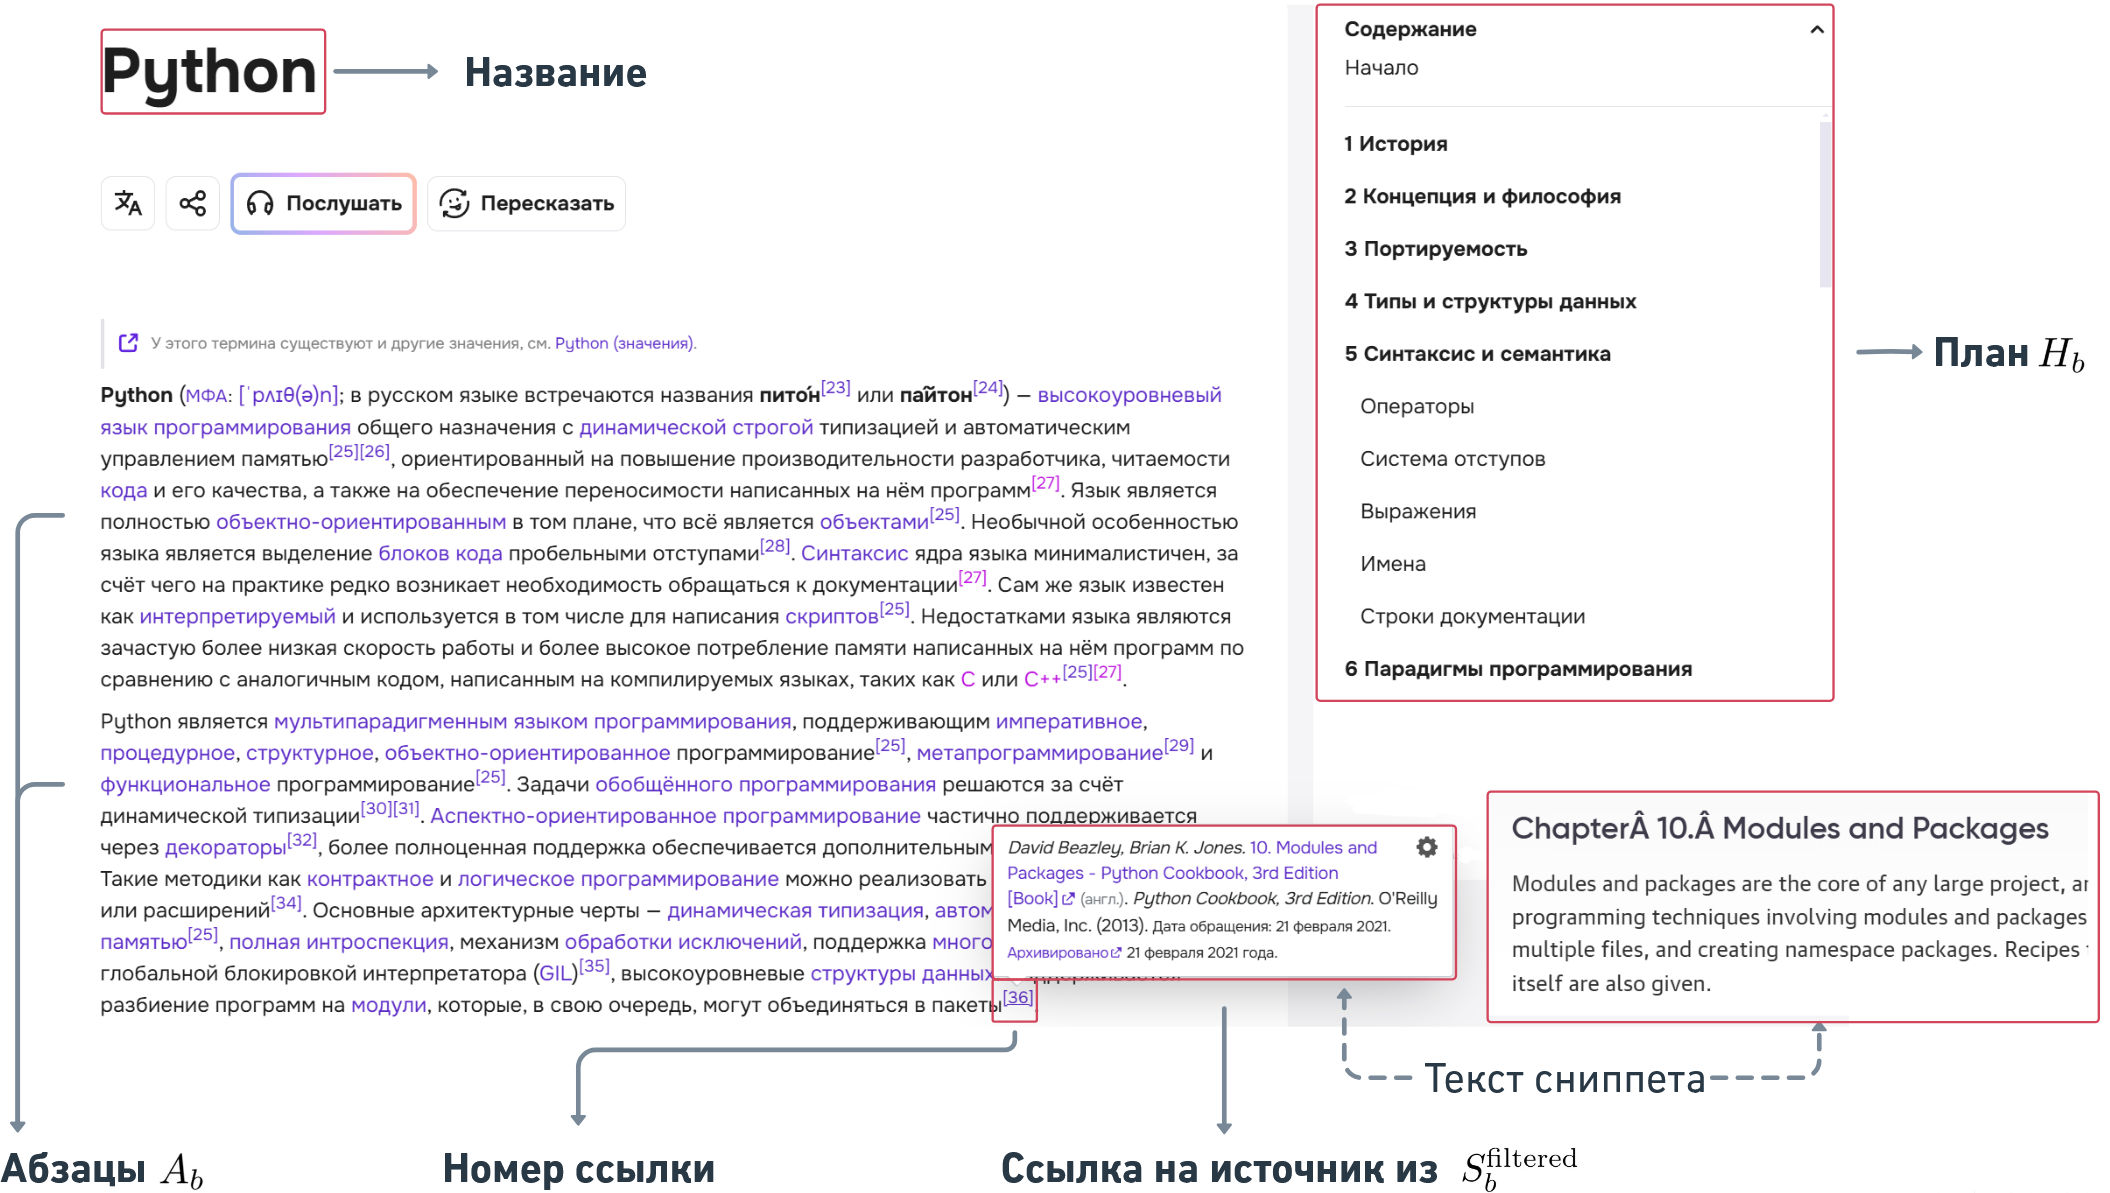
\includegraphics[width=0.85\textwidth]{figures/article_entities.png}
  \caption{Основные сущности статьи}
  \label{fig:article}
\end{figure}

На этапе получения данных осуществляется первичное извлечение информации из выбранной статьи и сбор связанных с ней источников. На рисунке \ref{fig:source} показана краткая схема извлечения текстов источников, 
их загрузка производилась с помощью Python-модуля \texttt{newspaper3k}\footnote{\url{https://github.com/codelucas/newspaper}}.
В качестве исходного корпуса берется подмножество статей <<Рувики>> \(B\).
Извлечение HTML-кода статьи выполняется с помощью стандартных инструментов Python-модулей\footnote{\url{https://beautiful-soup-4.readthedocs.io/en/latest/}},\footnote{\url{https://requests.readthedocs.io/en/latest/index.html}}. 
Полученный текст структурируется путем разбиения на фрагменты, соответствующие вложенным заголовкам (H1, H2, H3 и т.д.), что позволяет сохранить как содержательную часть статьи, так и ее иерархическую организацию. 
Далее из раздела <<Примечания>> автоматически извлекаются все внешние ссылки, на которые ссылается статья. Недействительные ссылки (например, код 404) исключаются из дальнейшей обработки,
а связанный с ними текст удаляется, оставляя только те источники, которые действительно доступны.

Рисунок \ref{fig:article} иллюстрирует схематичное разбиение статьи\footnote{\url{https://ru.ruwiki.ru/wiki/Python}} на ключевые сущности, используемые в дальнейшей обработке.
На этапе обработки данных выполняется фильтрация текста для обеспечения его корректной интерпретации моделью. 
Каждая сноска (например, [1], [2]) сопоставляется с конкретной ссылкой, соответствующей одному из доступных источников. 
Это позволяет точно определить позицию ссылки в тексте статьи и использовать ее для последующей фильтрации. 

\begin{table}[ht!]
  \centering
  \caption{Основные характеристики собранного датасета}
  \label{tab:dataset}
  \begin{tabular}{lcc}
    \hline
    \textbf{Показатель} & \textbf{RuWikiBench} & \textbf{ResearchArena} \\
    \hline
    Количество статей                             & 285 & 7,952\\
    \hline
    Количество скачанных источников               & 15,686 & 12,034,505\\
    \hline
    Общее число сниппетов                         & 36,860 & -\\
    \hline
    Средний размер плана (число заголовков)       & 37 & -\\
    \hline
    Средний размер секции (число слов)            & 112 & -\\
    \hline
  \end{tabular}
\end{table}

На основании действительных ссылок \(S_b^{\mathrm{filtered}}\) формируются очищенные множества абзацев \(A_b^{\mathrm{filtered}}\) и заголовков \(H_b^{\mathrm{filtered}}\), 
то есть остается только контент, подкрепленный извлеченными источниками, все прочее удаляется. 
Сохраняются только источники, для которых удалось получить текст \(t_q\) объемом не менее 1500 символов,
чтобы отсечь <<шумовые>> ответы с HTML-страниц вроде ошибок (например, error 404) или сообщений о блокировке. 
В \(A_b^{\mathrm{filtered}}\) остаются только те абзацы, в которых присутствует хотя бы одна ссылка на источник, для которой был успешно получен текст.
Аналогично формируется \(H_b^{\mathrm{filtered}}\) - только те заголовки, под которыми остался хотя бы один абзац.
Характеристики собранного корпуса представлены в таблице \ref{tab:dataset}.

% МЕТОДИКА ОЦЕНКИ --------
\section*{Методика оценки}

Для объективной оценки способностей языковых моделей генерировать научно-энциклопедические тексты, необходимо воспроизвести реальный процесс подготовки энциклопедического контента:
\begin{enumerate}

    \item \textbf{Отбор релевантных источников}: модель получает заголовок статьи и набор сниппетов, среди которых необходимо идентифицировать и ранжировать по степени значимости материалы, соответствующие тематике; 
    
    \item \textbf{Построение структуры статьи}: на основании темы и отобранных источников модель формирует план с выделением основных разделов в стиле Википедии;
    
    \item \textbf{Генерация секций}: материалы статьи распределяются по разделам, после чего для каждого раздела порождается обобщение его релевантных материалов.

\end{enumerate}
Каждый этап оценивается независимо от предыдущих, что позволяет количественно измерить качество выполнения конкретной подзадачи. 
\subsection*{Отбор релевантных источников.}
Одной из наиболее эффективных стратегий поиска \cite{rerank} является предварительная генерация предполагаемого результата (описания) по исходному запросу (названию статьи) для создания расширенного запроса поиска.
Описание генерируется на русском и английском языках, так как тексты источников тоже представлены в двух языковых вариантах. 
Запросы на обоих языках далее объединяются в единый текстовый запрос к системе поиска, основанной на BM25. 

Проводились эксперименты с двумя вариантами составления запроса:
\begin{enumerate}

    \item \textbf{Заранее сгенерированный запрос по названию и заголовкам второго уровня}: позволяет провести чистую оценку способностей ранжирования моделей; для генерации запроса применялась модель LLaMa 3 70b;
    
    \item \textbf{Запрос, сгенерированный по названию посредством оцениваемой модели}: подобно реальным условиям, LLM полностью отвечает за качество выдачи и самостоятельно решает, какой поисковый запрос лучше сформулировать для BM25.

\end{enumerate}
Примеры порождаемых описаний приведены на рисунке \ref{fig:cxx}.

\begin{figure}[ht!]
  \centering
  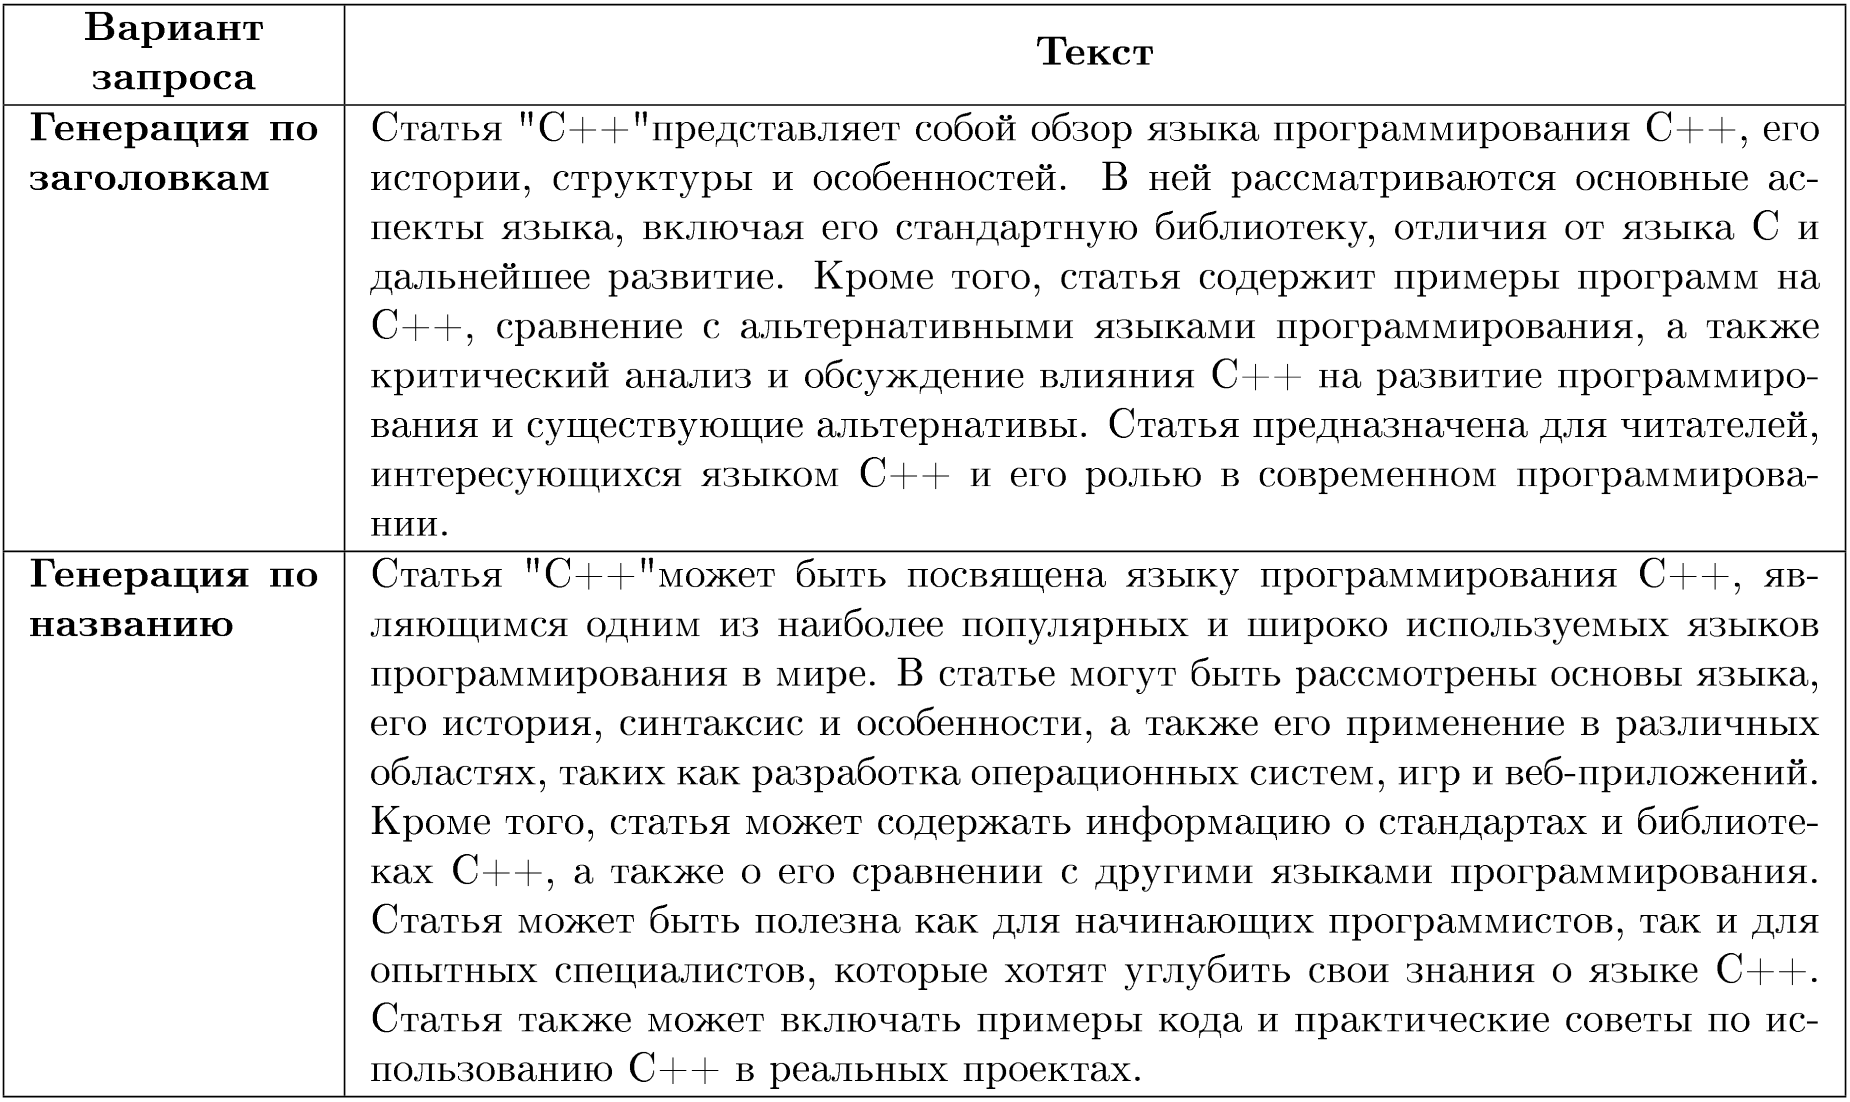
\includegraphics[width=\textwidth]{figures/two_queries.png}
  \caption{Сравнение описаний статьи <<C++>> в двух вариантах}
  \label{fig:cxx}
\end{figure}

Отобранные по запросу BM25 документы последовательно передаются большой языковой модели, которая должна определить каждый сниппет как релевантный (ответ <<да>>) или нерелевантный (ответ <<нет>>). 
Для получения численных оценок сравниваются названия статей, к которым относятся документы из выдачи и название статьи, для которой происходит отбор текстов-источников. 
Берется логарифмическая вероятность токенов в ответе модели: если это был утвердительный ответ, то берется сама вероятность $P(\text{да})$, если отрицательный, то $1 - P(\text{нет})$.
Такой подход позволяет ранжировать выдачу документов по уверенности модели в релевантности: чем выше вероятность, тем выше степень уверенности модели в ответе, тем выше документ будет в выдаче.

\subsection*{Построение структуры статьи.}
Сначала каждый текстовый фрагмент (сниппет) эталонного источника статьи преобразуется в векторное представление с использованием выбранной модели эмбеддингов. 
Затем сниппеты разбиваются на кластеры - потенциальное содержание секций. 
Для детерминированности, применяется алгоритм KMeans с числом кластеров равным числу заголовков 2го уровня эталонного плана и инициализацией центроидов векторными представлениями этих заголовков. 

Далее отбираются пять сниппетов, наиболее близких к центру кластера. Это делается с целью снизить влияние менее релевантных сниппетов на итоговый план. 
Формирование мини-планов секций осуществляется с учетом двух ключевых параметров: 
размера окна контекста (для учета отсылок и общей семантики документа) и двух режимов генерации - напрямую по текстам и через предварительную генерацию краткого описания кластера.
Два режима генерации позволяют выбирать уровень абстракции: 
прямой режим сохраняет детали при необработанных данных, а режим через предварительное описание кластера
повышает согласованность формулировок и уменьшает дублирование информации.
На заключительном этапе происходит объединение всех мини-планов в итоговый структурированный план статьи.

\subsection*{Генерация секций.}
Для каждой секции статьи извлекаются все сниппеты, которые указывались в качестве источников к эталонному тексту секции. 
Все сниппеты снова переводятся в эмбеддинги и строится матрица попарных сходств как произведение \(Emb \times Emb^\top\).
Элементы со значением сходства выше порога 0.8 (значение подобрано эмпирически) считаются близкими по смыслу и объединяются в группы, 
чтобы избежать избыточных повторов при генерации (например, когда разные источники перефразируют одно и то же). 
Для каждой такой смысловой группы строится иерархическое представление: берутся первые пять текстов, по ним генерируется краткое описание, 
затем это описание дополняется на основе следующих пяти и так далее, пока не получено полное сжатое представление группы.
Таким образом остается только некоторый набор кратких описаний - самая важная информация без лишних повторов.
После этого по полученным описаниям групп генерируется текст секции с использованием иерархического метода реферирования \cite{hier}.

% ОПИСАНИЕ ПАРАМЕТРОВ ЭКСПЕРИМЕНТА --------
\section*{Описание параметров эксперимента}
Ниже приведено описание всех использованных данных, моделей, гиперпараметров и процедуры для обеспечения воспроизводимости и анализа.

\subsection*{Параметры генерации.}
Для всех моделей, если не указано иное, использовались одинаковые параметры генерации: температура - 0.01, коэффициент штрафа за повторения - 1.0 и значение top\_p - 0.9.

\subsection*{Отбор релевантных источников.}
Индексирование сниппетов производится с помощью BM25\footnote{\url{https://github.com/xhluca/bm25s}} по всему корпусу собранных сниппетов без настройки гиперпараметров (стандартные значения).
Для каждого релевантного документа выбираются два нерелевантных (соотношение 1:2) - это сделано для повышения устойчивости оценки.

\subsection*{Построение структуры статьи.}
Сниппеты переводились в векторное пространство с помощью модели \texttt{sergeyzh/BERTA}\footnote{\url{https://huggingface.co/sergeyzh/BERTA}}. 
Рассматривались два варианта контекстного окна: используется либо нулевое окно (только сам сниппет), либо по одному соседнему сниппету слева и справа для расширения контекста.  

Схожесть заголовков с эталонными сравнивалась при помощи косинусной близости: учитывалось именно смысловое соответствие, а не точная формулировка или уровень заголовка. 
Сравнение проводилось с очищенной структурой статьи: из предобработанного текста удалялись все заголовки, секции которых полностью состояли из текста без доступных для скачивания источников. 

% МЕТРИКИ ОЦЕНКИ КАЧЕСТВА --------
\section*{Метрики оценки качества}

В рамках бенчмарка применяются две группы метрик: метрики ранжирования, оценивающие, насколько хорошо модель отбирает релевантные источники, и метрики схожести текста, измеряющие соответствие сгенерированного содержания эталонному.

\subsection*{Метрики ранжирования.}

Для оценки качества списка источников используются \textbf{NDCG@\textit{K}} \cite{ndcg}, и $\mathrm{R\text{-}Precision}$ \cite{rprecision}:
\begin{equation}\label{ndcg}
\mathrm{NDCG@K}= \frac{\mathrm{DCG@K}}{\mathrm{IDCG@K}}
\end{equation}

\begin{equation}\label{dcg}
\mathrm{DCG@K}= \sum_{i=1}^{K} \frac{\mathrm{rel}_i}{\log_2(i+1)}
\end{equation}

\begin{equation}\label{idcg}
\mathrm{IDCG@K}= \sum_{i=1}^{K} \frac{\mathrm{rel}^{\mathrm{IDEAL}}_i}{\log_2(i+1)}
\end{equation}

\begin{equation}\label{rpr}
\mathrm{R\text{-}Precision}= \frac{\sum_{i=1}^{R} \mathrm{rel}_i}{R}
\end{equation}

где \(\mathrm{rel}_i\in\{0,1\}\) - индикатор релевантности документа на позиции \(i\); \(\mathrm{rel}^{\mathrm{IDEAL}}_i\) - та же величина в идеальной (полностью отсортированной) выдаче;  
\(R\) - общее число релевантных документов для данного запроса.  

\subsection*{Метрика схожести текста.} 
Качество сгенерированных секций и заголовков оценивается \\\textbf{BERTScore} \cite{bertscore}:

\begin{equation}\label{recall}
R_{\mathrm{BERT}}= \frac{1}{|x|}\sum_{x_i\in x}\max_{\hat{x}_j\in\hat{x}} x_i^\top \hat{x}_j
\end{equation}

\begin{equation}\label{precision}
P_{\mathrm{BERT}}= \frac{1}{|\hat{x}|}\sum_{\hat{x}_j\in\hat{x}}\max_{x_i\in x} x_i^\top \hat{x}_j
\end{equation}

\begin{equation}\label{f}
F_{\mathrm{BERT}}= \frac{2\,P_{\mathrm{BERT}}\,R_{\mathrm{BERT}}}{P_{\mathrm{BERT}} + R_{\mathrm{BERT}}}
\end{equation}

где \(x\) - эталонный текст, \(\hat{x}\) - сгенерированный; каждое предложение кодируется с помощью модели\footnote{\url{https://huggingface.co/sergeyzh/BERTA}}, после чего вычисляется косинусное сходство.  

Для оценки генераций секций также рассматривались ROUGE-\allowbreak L и BLEU.

\textbf{ROUGE-L} \cite{rouge} - основана на длине наибольшей общей подпоследовательности (LCS) между сгенерированным рефератом $S$ и эталонным $R$.
Вычисляется по формуле \eqref{rouge} с использованием формул \eqref{r_p} и \eqref{r_r}:
\begin{equation}\label{r_p}
  \text{Precision} = \frac{\mathrm{LCS}(S,R)}{|S|},\quad
\end{equation}
\begin{equation}\label{r_r}
  \text{Recall} = \frac{\mathrm{LCS}(S,R)}{|R|}
\end{equation}
\begin{equation}\label{rouge}
  \text{ROUGE‑L} = \frac{2\;\text{Precision}\;\cdot\;\text{Recall}}{\text{Precision} + \text{Recall}}
\end{equation}

\textbf{BLEU} \cite{bleu} - метрика n-граммной точности с учетом штрафа за краткость. Итоговый счет определяется по формуле \eqref{bleu}:
\begin{equation}\label{bleu}
\mathrm{BLEU}_N = \mathrm{BP}\cdot \exp\!\left(\sum_{n=1}^{N} w_n \log p_n\right),
\end{equation}
где \(p_n\) - точность для \(n\)-грам, \(w_n\) - веса, $\mathrm{BP}$ - штраф за краткость.

% ОПИСАНИЕ РЕЗУЛЬТАТОВ ЭКСПЕРИМЕНТА --------
\section*{Описание результатов эксперимента}
\subsection*{Используемые модели.}
В экспериментах использовались следующие большие языковые модели: 
RuadaptQwen2.5-\allowbreak 7B-\allowbreak Lite-\allowbreak Beta \cite{ruadapt},
RuadaptQwen3-\allowbreak 32BInstruct-v2 \cite{ruadapt}, 
DeepSeek V3 \cite{deepseek}, 
Qwen3-\allowbreak 235B-\allowbreak A22B \cite{qwen3}, 
tpro \cite{tpro} и yagpt5lite \cite{yagpt}.
Во всех таблицах модели упорядочены по размеру, а наилучшие результаты внутри каждой весовой группы выделены.

\subsection*{Полученные результаты.}
В таблицах \ref{tab:query_ref} и \ref{tab:query_def} представлены результаты измерения качества ранжирования. 
Также были добавлены результаты бейзлайна, в качестве которого выступала выдача BM25 без переранжирования с помощью моделей. 
В первом случае (таблица \ref{tab:query_ref}), когда для всех моделей использовался заранее сгенерированный поисковый запрос, 
лучшие результаты показала модель DeepSeek V3, что свидетельствует о ее высокой способности отбирать релевантные документы.
Во втором эксперименте (таблица \ref{tab:query_def}), где запрос формировался только на основе названия статьи, tpro показала лучшие результаты. 
Эксперимент показал, что самостоятельная генерация запроса BM25 не уступает по качеству ранжирования эталонному варианту, в котором запросы генерируются более <<сильной>> моделью и затем
используются всеми оцениваемыми моделями. Предположительно, это связано с тем, что, как показано на рисунке \ref{fig:cxx}, запросы получаются похожими, потому что
LLM имеют представления о типовой структуре статьи Википедии из обучения и поэтому умеют связывать релевантные концепты в нужном формате.

\begin{table}[ht!]
\centering
\caption{Результаты чистой оценки навыков ранжирования}
\begin{tabular}{l|c|c}
\hline
\textbf{Model} & \textbf{NDCG} & \textbf{R‑Pr} \\
\hline
baseline (bm25)                                     & 88.81 & 62.51 \\
\hline
\textbf{DeepSeek V3}                                & \uline{\textbf{95.42}} & \uline{\textbf{83.86}} \\
Qwen3-235B-A22B                                     & 94.49 & 82.42 \\
\hline
RuadaptQwen3-32B-Instruct-v2                        & 95.25 & 81.81 \\
tpro                                                & \uline{95.42} & \uline{83.53} \\
\hline
RuadaptQwen2.5-7B-\allowbreak Lite-\allowbreak Beta & 88.26 & 62.26 \\
yagpt5lite                                          & \uline{90.35} & \uline{77.66} \\
\hline
\end{tabular}
\label{tab:query_ref}
\end{table}

\begin{table}[ht]
\centering
\caption{Результаты оценки навыков генерации запроса BM25}
\begin{tabular}{l|cc|cc}
\hline
\multirow{2}{*}{\textbf{Model}} & \multicolumn{2}{c|}{\textbf{BM25}} & \multicolumn{2}{c}{\textbf{Rerank}} \\
 & \textbf{NDCG} & \textbf{R-Pr} & \textbf{NDCG} & \textbf{R-Pr} \\
\hline
DeepSeek V3                                         & 88.39 & 60.65 & \uline{95.67} & \uline{83.07} \\
Qwen3-235B-A22B                                     & \uline{89.17} & \uline{62.98} & 94.90 & 81.96 \\
\hline
RuadaptQwen3-32B-Instruct-v2                        & 85.39 & 52.80 & 95.82 & 81.62 \\
\textbf{tpro}                                       & \uline{\textbf{90.61}} & \uline{\textbf{65.07}} & \uline{\textbf{96.06}} & \uline{\textbf{83.37}} \\
\hline
RuadaptQwen2.5-7B-\allowbreak Lite-\allowbreak Beta & \uline{88.81} & \uline{62.51} & 88.23 & 60.96 \\
yagpt5lite                                          & 86.59 & 57.98 & \uline{90.27} & \uline{77.65} \\
\hline
\end{tabular}
\label{tab:query_def}
\end{table}

В целом, модели демонстрируют достаточно высокие значения метрик на данном этапе, что может быть обусловлено тем, что название статьи хорошо отражает ее содержание. 
В лучших случаях до 80\% документов в выборке являются релевантными, что можно считать хорошим показателем, однако остается потенциал для дальнейшего улучшения.

\begin{table}[ht!]
\centering
\caption{Результаты генерации планов}
\begin{tabular}{l|c|c|c}
\hline
\multirow{2}{*}{\textbf{Model}} & \multicolumn{3}{c}{\textbf{Mean BERTScore F1}} \\
\cline{2-4}
 & \textbf{Default} & \textbf{Description} & \makecell{\textbf{Default with} \\ \textbf{one neighbor}} \\
\hline
DeepSeek V3                                         & \uline{\textbf{63.51}} & \uline{\textbf{65.50}} & \uline{\textbf{62.93}} \\
Qwen3-235B-A22B                                     & 60.86 & 62.66 & 59.06 \\
\hline
RuadaptQwen3-\allowbreak 32BInstruct-v2             & 60.12 & \uline{62.91} & \uline{60.04} \\
tpro                                                & \uline{60.32} & 60.75 & 59.09 \\
\hline
RuadaptQwen2.5-7B-\allowbreak Lite-\allowbreak Beta & \uline{60.03} & \uline{61.58} & 58.21 \\
yagpt5lite                                          & 59.72 & 60.25 & \uline{60.07} \\
\hline
\end{tabular}
\label{tab:outline_res}
\end{table}

В таблице \ref{tab:outline_res} представлены результаты оценки качества построения структуры статьи. Результаты показывают, что при предварительной генерации описания (режим Description) 
качество работы всех моделей стабильно повышается. 
Наибольший прирост демонстрирует модель RuadaptQwen3, поднимаясь на второе место, фактически сравниваясь по результатам с более крупной моделью
- Qwen3-\allowbreak 235B-\allowbreak A22B. Лидером остается DeepSeek V3, показывая значительный отрыв от остальных. На последнем месте по качеству находятся модели RuadaptQwen2.5-7B-\allowbreak Lite-\allowbreak Beta и yagpt5lite.
При этом yagpt5lite, имея всего 8 млрд., показывает результаты сопоставимые с моделью объемом 32 млрд. параметров.
На рисунке \ref{fig:outline} приведено сравнение небольшого отрывка эталонного и сгенерированного планов.
Получившиеся результаты хорошо коррелируют со степенью сходства заголовков с эталонными. Общей проблемой всех моделей была чрезмерная глубина иерархии заголовков.
На <<Рувики>> заголовки редко были глубже третьего уровня, однако модели часто создавали и четвертый, и пятый, подразумевая, что вся информация находится в одной большой секции, хотя
она может несколько отличаться по смыслу и в оригинальном плане это были бы не связанные заголовки.

\begin{figure}[ht!]
  \centering
  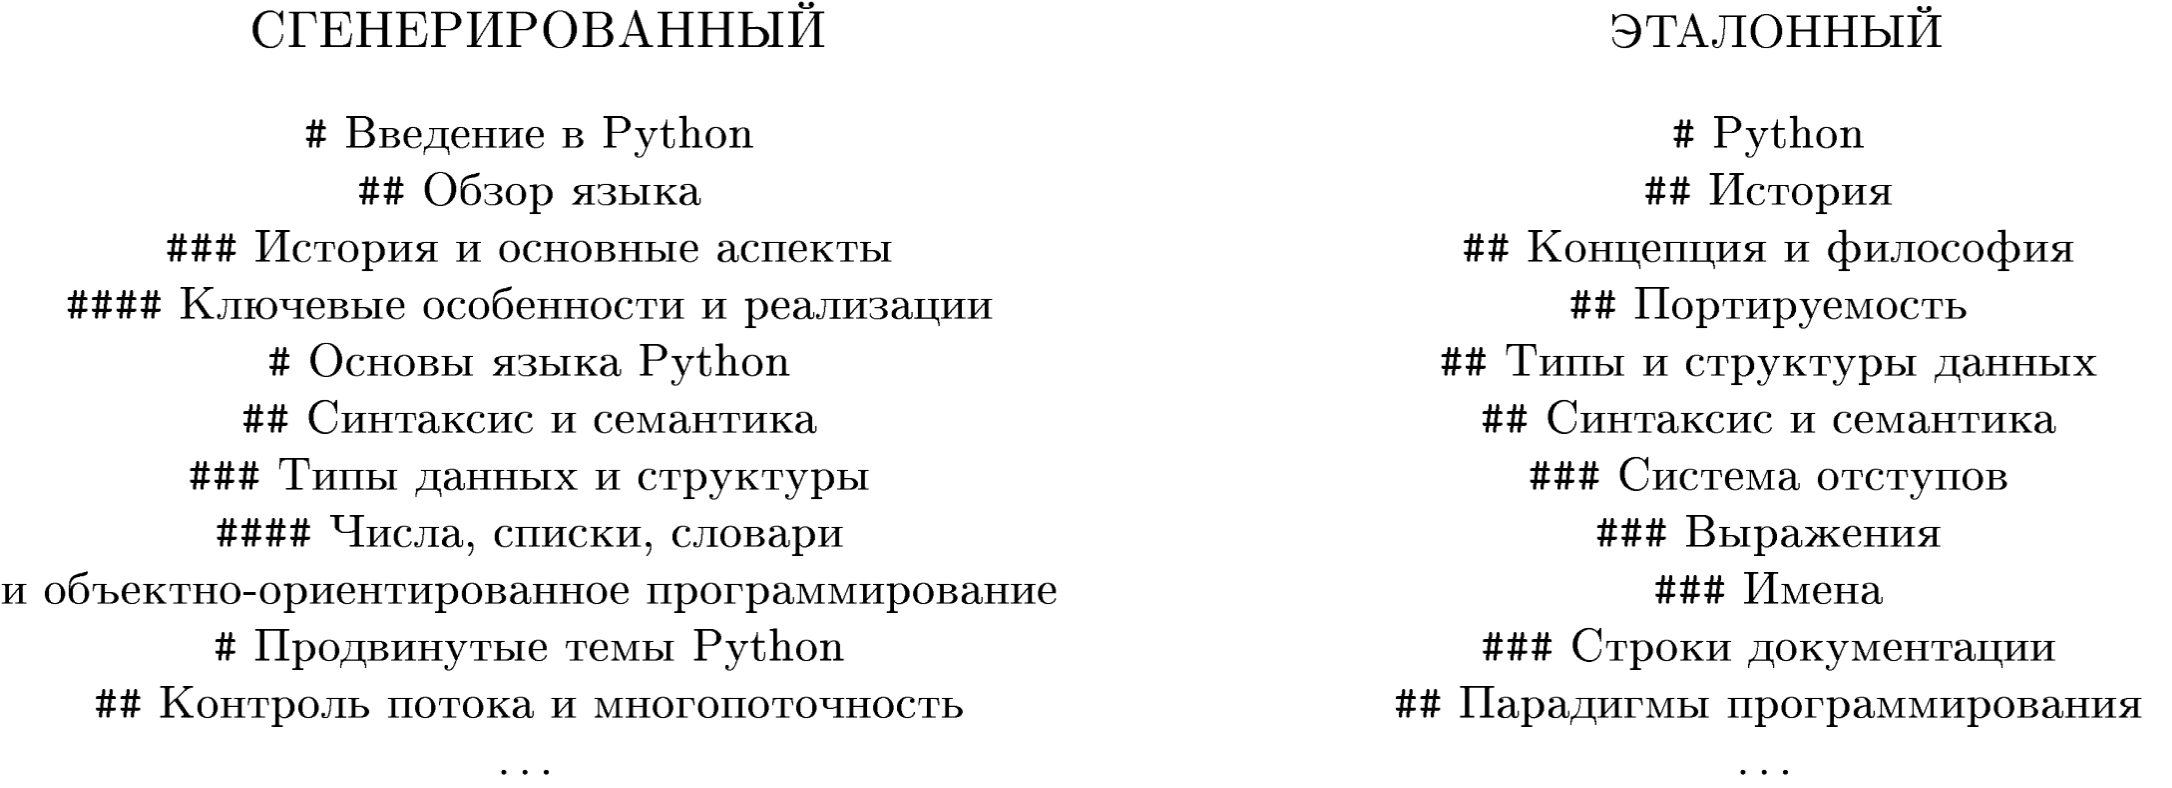
\includegraphics[width=\textwidth]{figures/outline.png}
  \caption{Сравнение двух планов статей}
  \label{fig:outline}
\end{figure}

В таблице \ref{tab:secs} приведены результаты замеров качества генераций секций. Итоговые результаты находятся на одном уровне, однако это обусловлено чувствительностью используемой метрики.
В итоговые метрики не вошли секции, для которых алгоритмом не было отобрано ни одного релевантного сниппета. Лучшие результаты 
продемонстрировала модель Qwen3-\allowbreak 235B-\allowbreak A22B, однако по метрикам ROUGE-\allowbreak L и BLEU лидирует RuadaptQwen3-\allowbreak 32BInstruct-v2, что говорит о лучшей структурной согласованности и 
большем совпадении формулировок с эталоном.
Модель yagpt5lite показывает результаты выше среднего, особенно по BLEU, при существенно меньшем размере, тогда как tpro демонстрирует минимальные значения по всем метрикам.

\begin{table}[ht!]
\centering
\caption{Результаты генерации секций}
\begin{tabular}{l|c|c|c}
\hline
\textbf{Model} & \textbf{Mean F1} & \textbf{Mean ROUGE-L} & \textbf{Mean BLEU} \\
\hline
DeepSeek V3                                         & 53.48 & 14.34 & 2.81 \\
Qwen3-235B-A22B                                     & \uline{\textbf{53.74}} & \uline{14.63} & \uline{3.07} \\
\hline
RuadaptQwen3-32B-Instruct-v2                        & 53.21 & \uline{\textbf{15.46}} & \uline{\textbf{3.40}} \\
tpro                                                & 53.15 & 13.58 & 2.27 \\
\hline
RuadaptQwen2.5-7B-\allowbreak Lite-\allowbreak Beta & 52.99 & 12.29 & 2.11 \\
yagpt5lite                                          & \uline{53.43} & \uline{14.85} & \uline{3.16} \\
\hline
\end{tabular}
\label{tab:secs}
\end{table}

Для наглядного сравнения качества генерации секций можно рассмотреть вводные части статьи <<COVID19>>, 
созданные моделями DeepSeek V3 и yagpt5lite соответственно, которые представлены на рисунке \ref{fig:secs_com}.
Несмотря на отдельные смысловые неточности (например, утверждение <<COVID-19 - это пандемия>>, тогда как в действительности речь идет о заболевании), 
модель yagpt5lite демонстрирует вполне достойный результат. Ее текст уступает варианту от DeepSeek V3 в части полноты охвата темы и системности изложения, 
но содержит больше числовых данных и конкретных фактов. При этом материал, сгенерированный DeepSeek V3, воспринимается как выдержка из энциклопедической статьи, 
тогда как версия yagpt5lite ближе по стилю к техническому отчету о заболевании.

\begin{figure}[ht!]
  \centering
  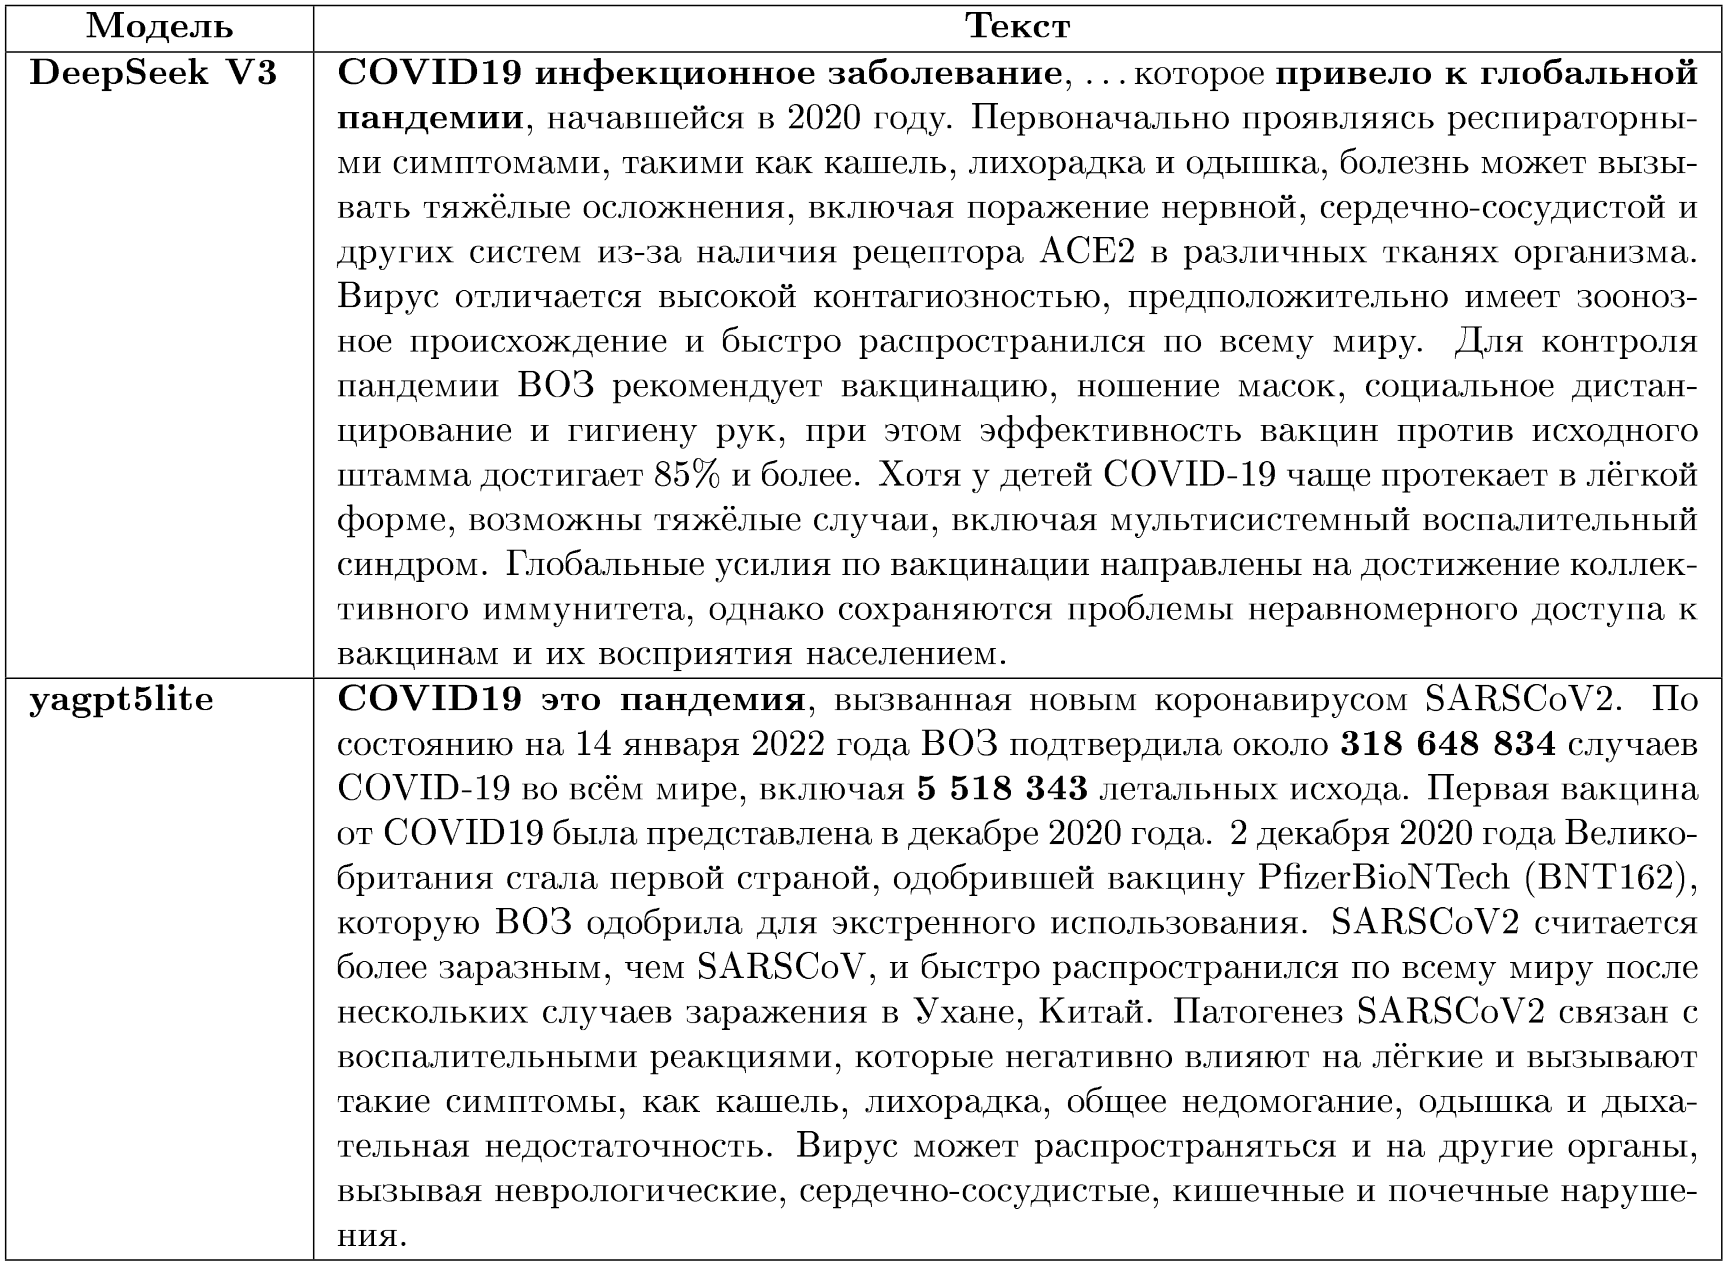
\includegraphics[width=0.9\textwidth]{figures/two_secs.png}
  \caption{Сравнение текстов двух секций}
  \label{fig:secs_com}
\end{figure}

% ЗАКЛЮЧЕНИЕ --------
\section*{Заключение}
В заключение, в работе предложен и реализован бенчмарк RuWikiBench для оценки аналитических способностей больших языковых моделей при генерации научно-энциклопедических текстов на русском языке.
В основу поставленной системы оценки лег трехэтапный процесс, состоящий из трех независимых систем, естественным образом возникающих при создании статей на определенную тему.
Опираясь на отфильтрованный корпус <<Рувики>> с сопоставленными сниппетами и четко определенной методикой оценки, 
предложенный бенчмарк создает основу для дальнейших исследований в области применения языковых моделей к задачам генерации научно-энциклопедического текста. 

Эксперименты показали, что при фиксированном поисковом запросе наилучшее качество отбора источников демонстрирует DeepSeek V3, 
заметно опережая BM25 без переранжирования.
На этапе построения структуры обнаружилось, что добавление предварительного описания кластера стабильно улучшает качество планов у всех моделей, включая DeepSeek V3, который продемонстрировал лучшее понимание процесса.
Все модели показали сравнимое качество генерации текста, однако по метрикам ROUGE-L и BLEU лидирует RuadaptQwen3-\allowbreak 32BInstruct-v2, что указывает на более согласованную с эталоном структуру текста.
Работа показывает, что модели обладают значительным потенциалом, 
но для их надежного применения требуется дальнейшая проработка методов анализа и структурирования обзорных материалов.

\section*{Благодарности}
Исследование выполнено за счет гранта Российского научного фонда № 25-11-00191, \url{https://rscf.ru/project/25-11-00191/}.

Работа выполнялась с использованием суперкомпьютера <<МГУ-270>> МГУ имени М.В. Ломоносова.

\begin{thebibliography}{99}

\bibitem{rsglue}
\textit{RussianSuperGlue.}
Shavrina T. et al. RussianSuperGLUE: A Russian language understanding evaluation benchmark //EMNLP 2020-2020 Conference on Empirical Methods in Natural Language Processing, Proceedings of the Conference. - 2020. - С. 4717-4726.

\bibitem{mera}
\textit{Mera.}
Fenogenova A. et al. MERA: A Comprehensive LLM Evaluation in Russian //Proceedings of the 62nd Annual Meeting of the Association for Computational Linguistics (Volume 1: Long Papers). - 2024. - С. 9920-9948.

\bibitem{libra}
\textit{LIBRA.}
Churin I. et al. Long Input Benchmark for Russian Analysis //CoRR. – 2024.

\bibitem{arena}
VikhrModels. RuLLM Arena: Russian LLM Evaluation Benchmark // GitHub repository. – URL: \url{https://github.com/VikhrModels/ru_llm_arena} (дата обращения: 01.08.2025).

\bibitem{pp}
\textit{Ping-Pong.}
Gusev I. PingPong: A Benchmark for Role-Playing Language Models with User Emulation and Multi-Model Evaluation.

\bibitem{deepr}
\textit{OpenAI.}
Introducing deep research // OpenAI URL: \url{https://openai.com/index/introducing-deep-research/} (дата обращения: 31.07.2025).

\bibitem{storm}
\textit{Storm.}
Shao Y. et al. Assisting in Writing Wikipedia-like Articles From Scratch with Large Language Models //NAACL-HLT. - 2024

\bibitem{resar}
\textit{ResearchArena.}
Kang H., Xiong C. ResearchArena: Benchmarking LLMs' Ability to Collect and Organize Information as Research Agents //arXiv e-prints. - 2024. - С. arXiv: 2406.10291.

\bibitem{rerank}
\textit{Reranking.}
Wang X. et al. Searching for Best Practices in Retrieval-Augmented Generation //CoRR. - 2024.

\bibitem{hier} 
Wu J. et al. Recursively Summarizing Books with Human Feedback //arXiv e-prints. - 2021. - С. arXiv: 2109.10862.

\bibitem{ndcg}
\textit{NDCG.}
Järvelin K., Kekäläinen J. Cumulated gain-based evaluation of IR techniques //ACM Transactions on Information Systems (TOIS). - 2002. - Т. 20. - №. 4. - С. 422-446.

\bibitem{rprecision}
\textit{R-Precision.}
BUCKLEY C. Evaluating Evaluation Measure Stability //ACM SIGIR 2000 Proceedings. - 2000.

\bibitem{bertscore}
\textit{BERTScore.}
Zhang T. et al. BERTScore: Evaluating Text Generation with BERT //International Conference on Learning Representations.

\bibitem{rouge}
\textit{ROUGE.}
Lin C. Y. Rouge: A package for automatic evaluation of summaries //Text summarization branches out. - 2004. - С. 74-81.

\bibitem{bleu}
\textit{BLEU.}
Papineni K. et al. BLEU: a Method for Automatic Evaluation of Machine Translation.

\bibitem{ruadapt}
\textit{RuadaptQwen.}
Tikhomirov M., Chernyshev D. Facilitating large language model russian adaptation with learned embedding propagation //Journal of Language and Education. - 2024. - Т. 10. - №. 4 (40). - С. 130-145.

\bibitem{deepseek}
\textit{DeepSeek V3.}
Liu A. et al. DeepSeek-V3 Technical Report //CoRR. - 2024.

\bibitem{qwen3}
\textit{Qwen3-235B.}
Yang A. et al. Qwen3 technical report //arXiv preprint arXiv:2505.09388. - 2025.

\bibitem{tpro}
Т-Банк открыл доступ к собственной русскоязычной языковой модели в весовой категории 7-8 млрд параметров // Т-Банк URL: \url{https://www.tbank.ru/about/news/20072024-t-bank-opened-access-its-own-russian-language-language-model-weight-category-of-7-8-billion-parameters/} (дата обращения: 10.05.2025).

\bibitem{yagpt}
YandexGPT 5 с режимом рассуждений // Яндекс URL: \url{https://ya.ru/ai/gpt} (дата обращения: 30.07.2025).

\end{thebibliography}

\end{document}